%!TEX root = ../dissertation.tex

\chapter{Embedded reconstruction of local primitives}
\label{chp:retina}
%\epigraph{We here propose to do just what Copernicus did in attempting to explain the celestial movements. When he found that he could make no further progress by assuming that all the heavenly bodies revolved round the spectator, he reversed the process and tried the experiment of assuming the spectator revolved, while the stars remained at rest.}{Immanuel Kant, \textit{Critique of Pure Reason}}
%\textit{Iniziare la ricostruzione a tempo 0 in maniera embedded durante il readout}

The LHCb collaboration has made of ``real-time analysis" one of his trademark, being the first HEP experiment to implement a fully online software-based trigger with an offline-quality reconstruction level. However, even if the RTA project showed outstanding results, there are some issue to address. 
%this idea relies mostly on leveraging the power of parallel computing such as the one of GPUs. 

The "real-time" reconstruction described in Section \ref{sec:rta} essentially runs the same algorithms that would be used for offline reconstruction, but at a much faster speed. This acceleration relies mostly on leveraging the power of parallel computing in centralised servers such as the farm of GPUs or CPUs implemented in the Event Builder and Event Filter Farm.
At the core-level, the complete online reconstruction is resource-intensive and time-consuming, leading to potential bottlenecks in data processing, such as the one already experienced by storing data in a buffer awaiting for them to be processed by HLT$2$. This can lead to delays in the trigger system, forcing LHCb to implement a lighter processing stage in HLT$1$, which uses a reduced amount of information to alleviate processing load.
However, even this small amount of data requires computationally expensive procedures. For example, HLT$1$ processes a list of detector hits to extract tracks and primary vertices \cite{https://doi.org/10.5281/zenodo.8119731}. This process requires raw data (the list of detector hits) to be read and reassembled to extract meaningful information (the tracks and the PVs).
%We could reduce the amount of computation, if we develop algorithms that provide directly the required information directly in the readout of the detector.

To address these challenges, this chapter proposes a different approach: extracting meaningful information directly during detector readout to reduce the amount of data that must be processed. By doing this, the subsequent stages receive only the essential relevant information, reducing the need for additional computation. For example, instead of the list of hits that needs to be converted in tracks and PVs, we could directly directly provide HLT$1$ the mean interaction point. This idea is known as ``edge computing", where computational tasks are shifted from centralised servers to locations closer to the data source—such as near or directly within the detector. While this approach may sacrifice some flexibility, it could dramatically speed up processing and focus resources on the data that truly matters.
%This embedded approach helps streamline the reconstruction process, starting directly from the readout of the detector.
%The core idea of this chapter is to minimise the amount of data that must be processed by extracting meaningful information directly during detector readout. This way, subsequent stages receive precisely the information they require, eliminating the need for additional computation.
%This concept is called ``edge computing". This philosophy shifts computational tasks from centralised servers to locations closer to the data source, such as directly within or near the detector. The key principle is to start the reconstruction in an embedded way directly in the readout of the detector. 
%If smarter algorithms could be developed to directly exploit only the relevant information—e.g. luminosity, detector position, or beamline position—it would make the process more efficient by reducing unnecessary computation. 

%With Moore's Law showing signs of saturation, traditional centralised-based processing is becoming less viable for tasks that demand rapid and efficient computation. 

This chapter explores the concept of ``embedded local primitives," which are raw-like data points that align closely with the specific quantities that need to be measured. The central module for enabling this approach is the Field Programmable Gate Array (FPGA), which allows for rapid computation of these primitives. A prime example of how this technique is already aiding in event reconstruction is the FPGA-based VELO clustering. Developed as the first phase of the "Artificial Retina" tracking architecture, it finds two-dimensional clusters in the VELO detector and produces the primitives at the heart of this study.
%Finally, I will introduce the specific mother of all the primitives used in this thesis:

By counting clusters in specific regions on the VELO detector, we could implement other local primitives, the cluster counters. The cluster counters can be linearly combined to enable real-time measurements of luminosity, beamline position, and VELO detector position, as it will be presented in the next chapters. By embedding the computation of these quantities directly within the detector hardware, these counters offer a swift and efficient means of processing data on the spot, minimising latency and improving the speed and accuracy of crucial measurements. 
%In fact, the alignment constants are calculated only for a certain subset of the data, under the assumption of stability in time. However, if this stability is not verified, potential biases or systematic uncertainties could be added to the reconstructed events. For example, the parameters concerning VELO alignment represented the major contribution to the systematic uncertainty in the precise determination of the $B_S^0-\overline{B_S} ^0$ oscillation frequency~\cite{b0b0soscillation}.

\section[The Field Programmable Gate Array]{The Field Programmable Gate Array $\bigl($FPGA$\bigr)$}

In modern digital systems, traditional interconnected integrated circuits are becoming impractical due to their high cost, low efficiency, and reliability issues. Instead, many complex digital systems are implemented on custom integrated circuits designed for specific applications, known as Application Specific Integrated Circuits (ASICs). While ASICs are efficient for mass production, they lack flexibility, especially in experimental or research settings where design changes and rapid iterations are frequent. This is where Field-Programmable Gate Arrays (FPGAs) become invaluable.

FPGAs are integrated circuits that allow users to configure their internal connections, creating custom logic designs. Unlike CPUs and GPUs, which have fixed architectures and execute sequential instructions from memory, FPGAs consist of a matrix of programmable logic blocks that can be interconnected according to a user-defined design. This design can be constructed by the user with the help of hardware description languages (HDLs), like VHDL and Verilog. This unique characteristic makes FPGAs highly adaptable, enabling rapid prototyping and experimentation without the need for expensive custom ASIC fabrication.

Furthermore, FPGAs offer unique benefits through their architecture, where multiple tasks can be executed in parallel across different logic blocks. This parallelism significantly increases throughput, allowing for high-speed data processing. Additionally, FPGAs can include Hard Intellectual Property blocks, which are optimised for specific functions like memory or high-speed communication.

The low-latency data handling and parallel processing capabilities of FPGAs are the characteristics that make them an ideal candidate for the computation of embedded local primitives, which is the focus of this thesis.

The LHCb experiment relies extensively on FPGA produced by Altera, one of the leading FPGA manufacturers. The programmable logic blocks within Altera's FPGAs are called Adaptive Logic Modules (ALMs), including Lookup Tables (LUTs), full adders, D-type flip-flops, and multiplexers. These components can be configured to perform various digital logic functions, arithmetic operations, and data storage. The number of ALMs in an FPGA determines its processing capacity, with the devices used for the purposes of this thesis containing 427200 ALMs.




\section{RETINA}
%In the context of advancing technologies for real-time track reconstruction, the INFN-RETINA project has emerged with a focus on implementing an FPGA-based computing architecture inspired by mammalian brain early image reconstruction processes. Progressing beyond its initial research phase, for Run3 operations the project has now developed a demonstrator on real hardware for reconstructing data from the VELO. 
%The initial phase involving the reconstruction of particle hits out of the raw pixel data, is performed by means of a 2D cluster-finding algorithm implemented in the 52 readout FPGAs of the VELO, for a total of 104 parallel channels. Each channel further subdivides clusters among multiple parallel sub-channels. Utilizing a pipelined internal architecture, certain operations are executed swiftly "on the fly" for all hits detected in each event, without causing delays in data acquisition or requiring extensive computational resources, provided the firmware is appropriately designed. Notably, this efficiency is maintained despite an average hit rate of approximately $4 \cdot 10^{10}$/s, which may appear prohibitive for exhaustive processing.\\

The RETINA project\cite{Lazzari:2801062} is an initiative aimed at advancing technologies for real-time track reconstruction from raw hits data in high-energy physics experiments. This project leverages FPGAs in order to build a computing architecture with rapid, high-throughput data processing using a parallel processing pipeline inspired by mammalian brain pattern recognition. The project's design aligns with the concept of ``edge-computing," where the computational load is distributed across hardware components closer to the source of the data, reducing latency and easing the burden on central processing resources.


One of the key components of the RETINA project is the ``Artificial Retina"\cite{Ristori:2000vg}, a pattern-matching architecture inspired by biological visual processing. This architecture plays a critical role in the reconstruction of downstream tracks, which is challenging due to the high computational load and complexity of traditional HLT processes. The Artificial Retina is designed to recognise specific track patterns by comparing them to stored reference patterns, providing a non-binary response that varies depending on the distance from the stored patterns.

The RETINA project has achieved significant milestones, demonstrating \SI{40}{\mega\hertz} event throughput with sub-microsecond latency when applied to a generic 6-layer tracking system. The project has transitioned from the R\&D phase to the implementation of a realistic prototype for reconstructing tracks within the VELO acceptance under Run-3 conditions. Data from the VELO detector are sent in a parasitic stream to a facility called the Coprocessor Testbed, where innovative prototypes are being tested under realistic data acquisition conditions. This facility allows for further optimisation and validation of the Artificial Retina before full deployment in the LHCb experiment.

The process begins with a $2$D cluster-finding algorithm implemented in the 52 readout FPGAs of the VELO, for a total of 104 parallel channels. Each channel further subdivides clusters among multiple parallel sub-channels. The internal pipelined architecture enables swift execution of specific operations ``on the fly", without causing delays in data acquisition, even at high hit rates.

Within the RTA working group, RETINA’s goal is to enhance the overall processing power of LHCb by providing a real-time tracking device that operates alongside the traditional data acquisition system. This requires low latency and high throughput, both of which are achievable with FPGAs. The Downstream Tracker, a component of RETINA, receives hits from the SciFi detector in parallel to the main stream of data delivered to HLT$1$, allowing for more efficient reconstruction of downstream tracks.

%The integration of the RETINA-based Downstream Tracker into LHCb's data acquisition system requires special considerations\cite{Lazzari:2888549}. The most effective way to implement this integration is by installing the Tracking Boards within unused slots inside the Event Builder (EB) server nodes. The distribution network is established through high-speed optical links, allowing seamless data transmission between different components.



%Overall, the RETINA project represents a significant advancement in real-time track reconstruction, providing a flexible and efficient FPGA-based solution for high-energy physics experiments like LHCb. Its approach to embedded reconstruction and edge-computing paves the way for more efficient data processing and analysis, supporting the future of high-energy physics research.

\section{The Clustering}

The ``Artificial Retina" architecture relies on accurate hit coordinates on the VELO detector. However, the VELO does not inherently produce these coordinates but instead provides information on which pixels are active within an event. This subtle difference can have a significant impact on tracking performance.

When a particle strikes a detector layer, it can activate multiple adjacent pixels. If a tracking algorithm treats each of these pixels as a separate hit, the complexity of resolving hit combinations increases exponentially. This leads to the potential for reconstructing multiple tracks from different pixels activated by a single particle hit. The tracking algorithm can remove these redundant tracks, but this requires additional processing time and resources.

To avoid these issues, contiguous active pixels are grouped into clusters before tracking. The process of finding clusters on a $2$D detector at LHC rates is challenging, and there is limited literature on the topic. In LHCb's HLT$1$, clustering was originally intended to use around 17\% of its computing resources. However, since the ``Artificial Retina" operates before the trigger, it requires an independent clustering process. In order to do not reduces the FPGA resources available for tracking, the clustering task was implemented directly on the VELO's readout boards. This solution dedicates all the Tracking Boards' resources to tracking and reduces the load on the trigger farm by providing direct clusters to HLT.

To address these challenges, a FPGA-based clustering algorithm was developed capable of operating at a \SI{30}{\mega\hertz} event rate in real time, using a relatively modest amount of hardware resources. The typical cluster sizes for charged particles crossing VELO layers are small, with 96\% containing between one and four pixels. 
%Larger clusters typically result from merged hits or secondary emissions (e.g., $\delta$-rays). This property suggests that the FPGA clustering algorithm should be optimised for small clusters.

Given that the average number of clusters per event for a VELO sensor is around seven, the overall detector occupancy remains low. Each sensor contains approximately 197,000 pixels, yielding an expected occupancy rate of around 0.125\%\cite{Bediaga:2013tje}. This low occupancy rate implies that a single large matrix for the entire sensor may not be the most efficient approach. Instead, smaller matrices that dynamically map different sensor areas are preferred. This strategy allows for a reduction in hardware resource usage while maintaining effective clustering capabilities. The developed FPGA-based clustering algorithm is designed with these considerations in mind, providing a robust and efficient solution for the VELO detector's clustering needs.

\subsection*{The Algorithm}
This algorithm has specific features designed for the VELO detector but can be generalised for other silicon pixel detectors. One of the key concepts in this clustering approach is the use of "SuperPixels" (SPs), which are the readout format of the VELO, corresponding to aggregated groups of 4~×~2 pixels. Each SP contains information about which of the eight pixels was active, its coordinates, and whether any neighbouring SPs are active. If none of the surrounding SPs has active pixels, the current SP is flagged as isolated. This information is leveraged by both HLT and FPGA algorithms to optimise the clustering process, allowing for faster algorithms for isolated SPs. Notably, about 53\% of SPs are isolated.
%These SPs contain detailed information about pixel activity within each block and are grouped into 256-bit packets called frames, each containing eight SPs. To manage the flow of data and provide context for clustering, each packet contains specific signals, including Start Of Package (SOP), End Of Package (EOP), and Data Valid. The SOP signal indicates the beginning of a new event, while the EOP signal marks the end, with the Data Valid signal providing information about the validity of the SP data.

The Clustering algorithm operates in two different ways depending on the isolation flag of the SPs.
\subsubsection{Clustering resolved entirely with LUTs for isolated SPs}
Isolated SPs can only have a limited number of possible configurations due to their smaller size and lack of neighbouring activity. The clustering algorithm takes advantage of this by using a LUT that contains pre-calculated cluster centres for each possible SP configuration. With $2^8$ possible configurations, this LUT-based approach provides extremely fast processing with minimal logic resource usage.

When an isolated SP is identified, the algorithm looks up its pixel configuration in the LUT and retrieves the corresponding cluster centre-of-mass. Since isolated SPs can contain up to two clusters, the LUT also provides this information. This mechanism allows for efficient cluster resolution without extensive computations. Given the high probability of having isolated SPs, this approach significantly reduces the computational load.

\subsubsection{Clustering algorithm for Non-Isolated SPs}
For non-isolated SPs, the clustering algorithm uses a more complex approach, involving the parallel processing of multiple neighbour SPs. To manage this complexity, the process employs a two-stage algorithm\cite{Lazzari:2813167}:
\begin{enumerate}
    \item A matrix filling mechanism for identifying cluster candidates
    \item Cluster Regognition through Pattern Matching
\end{enumerate}

\paragraph{The matrix-filling mechanism}
This approach uses matrices of 3 rows and 3 columns, creating a 12~×~6 pixel structure that can contain multiple SPs. The matrices are not static, but they are dynamically filled based on the incoming SPs.

The first SP in a given event defines the center of a blank matrix, establishing the physical coordinates of that matrix within the VELO detector. Subsequent SPs fill the neighbouring cells if the Čebyšëv distance between them is 1 (i.e. their coordinates differ at most by 1). If an SP does not match any position in the matrix, it moves forward in a chain of matrices, eventually filling the centre of a new blank matrix. This process is repeated until all the SPs are processed.

Figure~\ref{fig:matrix_filling_clustering} illustrates this matrix-filling mechanism, demonstrating how SPs find their appropriate place in the matrix structure.

\begin{figure}
    \centering
    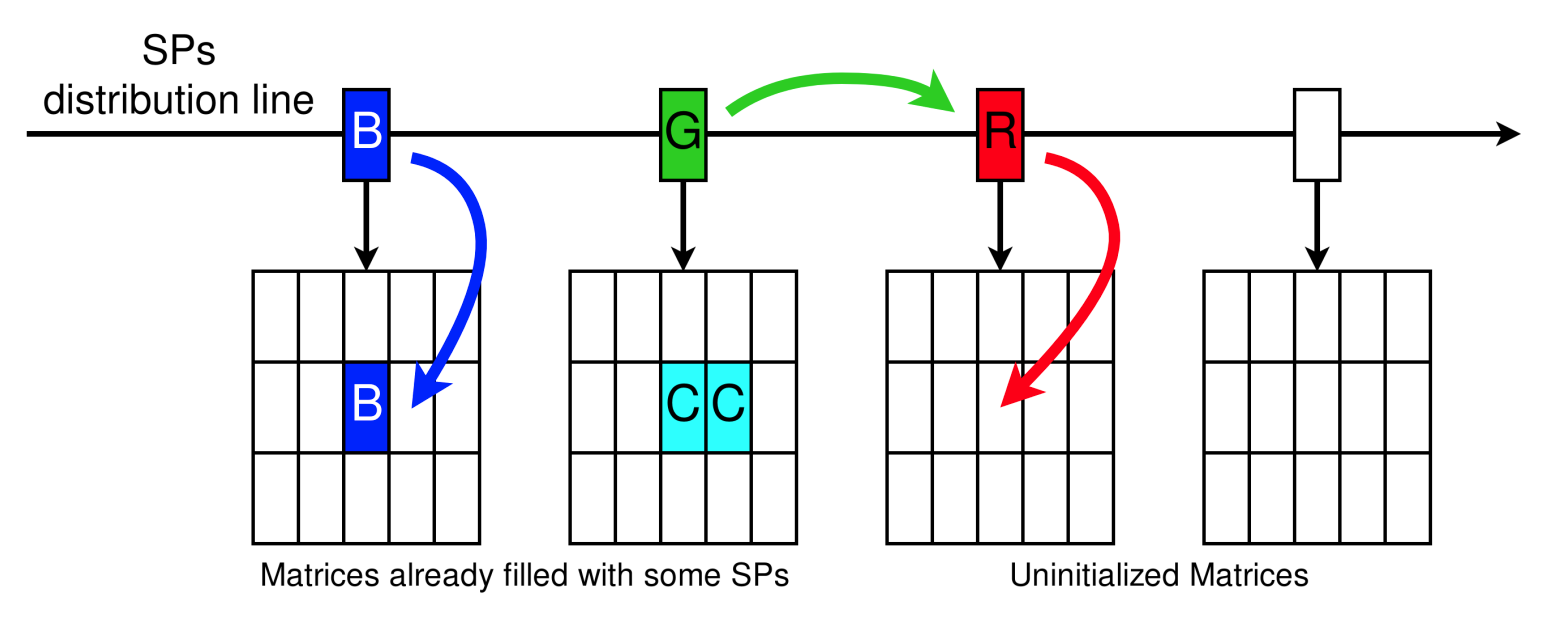
\includegraphics[width=\textwidth]{figures/matrix_filling_clustering.png}
    \caption{Matrix filling example for non isolated pixel. The horizontal line corresponds to the SPs distribution line, while squares of the same colour corresponds to adjacent SPs. The four matrices displayed correspond to two cases: the two on the left are already filled with some SPs, while the two on the right are uninitialised matrices. In this example, in the distribution line we read three different SP (which are blue, green and orange coloured for explanatory reasons). The blue superpixel is adjacent to the SP filling the matrix on the left, therefore it is added to that matrix. The green pixel checks if it belongs to the matrix below him, but since it is not adjacent to the SPs in that matrix, it is moved forward in the line. At the same time, the orange pixel fills an empty matrix since it did not find any adjacent pixel in the already filled matrices. Eventually, the green SP will also fill a blank matrix.}
    \label{fig:matrix_filling_clustering}
\end{figure}

\paragraph{Cluster Regognition through Pattern Matching}
As soon as the matrix filling is complete, the algorithm uses a pattern-matching technique to identify clusters in a complete parallel way. Each pixel within the matrix checks for specific patterns that signify cluster presence. The most common pattern involves an ``L" shape, where an inactive sequence of pixels surrounds an active pixel, providing a natural boundary. A second pattern, involving a diagonal arrangement of two active pixels, is used to identify clusters that might be missed by the first pattern. The combination of these patterns allows for high cluster recognition efficiency.

Once a pattern is matched, the cluster candidate is recognised within the 3~×~3 grid, as shown in Figure~\ref{fig:cluster_recognition}. The centre-of-mass of the cluster candidate is then calculated using a LUT with 512 entries, which provides the cluster absolute position. This position is determined based on the matrix location within the VELO detector and the cluster candidate position within the matrix.

\begin{figure}[h]
    \centering
    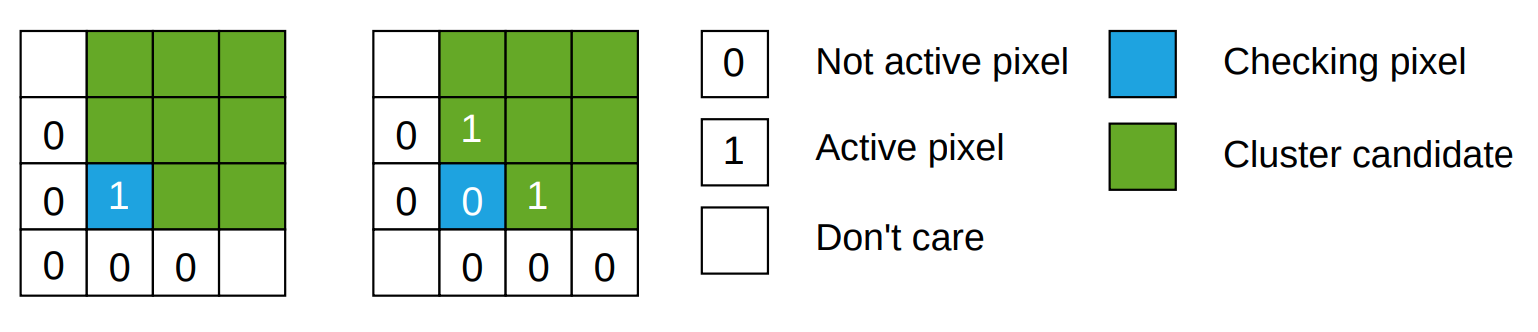
\includegraphics[width=\textwidth]{figures/cluster_recognition.png}
    \caption{Pixel patterns associated to clusters}
    \label{fig:cluster_recognition}
\end{figure}

\section{The VELO Cluster Counters}\label{sec:velo_counters}
%\textit{Definition of the selection regions, implementation of the counters on FPGA, counters per bxid, counters per bxtype}
Cluster counters on the VELO are critical components for generating the primitives used to estimate the experimental parameters studied in this thesis: luminosity, beamline position, and VELO position. 

The cluster counters are designed to count the number of clusters within specific regions of the VELO detector, providing fundamental data for further analysis. The firmware, following the clustering process, counts clusters in eight distinct selection regions within each of the 26 VELO stations, resulting in a total of 208 (8~×~26) individual counters. In Figure~\ref{fig:VELO-counters} we report a scheme of a VELO station with the position of the selection regions highlighted in red and black. Each one of these selection regions is located on a different sensor of the VELO and has dimension of 20~×~110 pixels. Specifically, the inner counters (red) cover the region between row 80 and row 100 and between column 620 and 730, while the outer counters (black) cover a region from row 20 to row 40 and from column 29 to column 139. This segmentation enables a detailed view of cluster distributions across the detector, offering valuable insights for the analysis of experimental events.% The choice of these selection region was done empirically, it is not assured that these region are the most sensible for the quantities to measure in this thesis. 


\begin{figure}
    \centering
    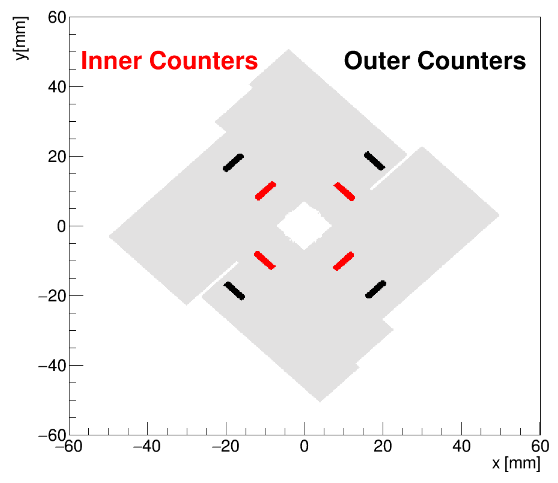
\includegraphics[width=0.6\textwidth]{figures/counters.png}
    \caption{A station of the VELO detector with the selection regions highlighted}
    \label{fig:VELO-counters}
\end{figure}

The cluster counters are configured to be read at an arbitrary frequency, allowing flexibility in data collection. In the current firmware implementation, these counters are read every three seconds, integrating information from approximately 120 million events. 
Each counter tracks the average number of clusters per event, ensuring that the total count is normalised by the number of events within the integration window. Furthermore, a running average is performed to guarantee continuity with consecutive readings of mean cluster counts.

To improve the accuracy of measurements and reduce noise from background events, the cluster counters differentiate between four types of bunch crossings: bunch-bunch (bb), bunch-empty (be), empty-bunch (eb), and empty-empty (ee). This distinction is important because it allows for the separation of proton-proton events (bb) from background events (be, eb, ee), where at least one of the colliding beam is empty, due to an empty bunch (indicated with the letter e). This information is carried out by a 2-bit signal in the TFC data sent by the clustering block firmware. In the TFC data also the bunch crossing ID (BXID) is also carried out.

Each one of the different bunch crossing counters is read and stored, but it is convenient to define already the cluster counter outputs used for the construction of the local primitives as: 
\begin{equation}
    c^i_{AVG} = c^i_{bb} - c^i_{be} - c^i_{eb} + c^i_{ee},
\end{equation}

where $i$ is index indicating the counter, spanning from 1 to 208, while the suffix refers to the bunch crossing type.

The information obtained from the 208 cluster counters forms the basis for building embedded primitives that are central to this thesis. These primitives are used to estimate luminosity, beamline position, and VELO position. The online background subtraction and ability to read cluster counts at a high frequency enable real-time data analysis, facilitating more accurate and timely estimates.

In the following chapters, I will explain how the cluster counters are utilised to create embedded estimators for these key parameters. 
%This process involves integrating the data from the counters, applying appropriate algorithms, and extracting meaningful information for further analysis. 